\section{Maxsus nisbiylik nazaryasi}



\begin{enumerate}

\item Maxsus nisbiylik nazariyasi -- bu fizikaning ... ni o‘rganadigan bo‘limidir.
\begin{enumerate}[label=\Alph*)]
\item yulduzlar va yulduzlar sistemalarini.
\item fazo va vaqtning asosiy hususiyatlarini.
\item qattiq jism tuzilishini.
\item atom tuzilishini.
\end{enumerate}

\item Keltirilgan tasdiqlardan qaysilarini nisbiylik nazariyasining postulatlari deb hisoblasa bo‘ladi?
\begin{itemize}
    \item[1)] har qanday inersial sanoq sistemada tabiatdagi barcha jarayonlar bir xilda yuz beradi;
    \item[2)] yorug‘likning vakuumdagi tezligi barcha inersial sanoq sistemalarda bir xildir;
    \item[3)] tabiatdagi barcha jarayonlar nisbiydir va har xil inersial sanoq sistemalarda har xil yuz beradi;
    \item[4)] yorug‘lik tezligi sanoq sistemaga bog‘liq.
\end{itemize}
\begin{enumerate}[label=\Alph*)]
\item 3, 4.
\item 1, 2.
\item 1.
\item 2.
\end{enumerate}

\item Quyidagilarning qaysilari nisbiylik nazariyasining asosiy postulatlandir?
\begin{itemize}
    \item[1)] tabiatdagi barcha jarayonlar har qanday inersial sistemada bir xilda yuz beradi;
    \item[2)] yorug‘likning vakuumdagi tezligi barcha inersial sistemalarda bir xildir. U manbaning harakat tezligiga ham, yorug‘likni qabul qilgichning tezligiga ham bog‘liq emas;
    \item[3)] fazoning turli joylarida sodir bo‘luvchi voqealarning bir vaqtda yuz berishi nisbiydir;
    \item[4)] jismlarning harakat yo‘nalishidagi o‘lchamlari nisbiydir.
\end{itemize}
\begin{enumerate}[label=\Alph*)]
\item 1, 2, 3, 4.
\item 2, 4.
\item 1, 2.
\item 2, 3, 4.
\end{enumerate}

\item Agar harakatlanayotgan jismning harakat yo‘nalishidagi uzunligi 40 foizga qisqargan bo‘lsa, uning tezligi qanday (m/s)?
\begin{enumerate}[label=\Alph*)]
\item $4\cdot 10^6$.
\item $6,4\cdot 10^6$.
\item $3,6\cdot 10^7$.
\item $2,4\cdot 10^8$.
\end{enumerate}

\item Rasmdagi to‘g‘ri to‘rtburchak $v = c/2$ tezlik bilan harakatlansa, uning yuzasi nimaga teng bo‘lib qoladi (m$^2$)?

\begin{center}
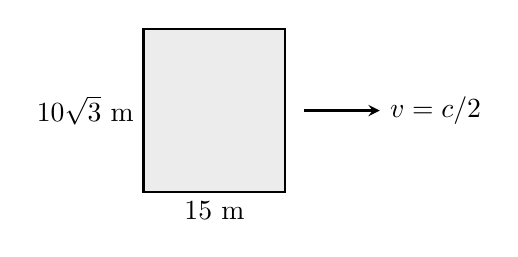
\begin{tikzpicture}[>=stealth, scale=1.2]
  % To'g'ri to'rtburchak
  \draw[thick, fill=gray!15] (0,0) rectangle (1.5, 1.73);
  % O'lchamlar va yozuvlar
  \node[left] at (0, 0.865) {$10\sqrt{3}$~m};
  \node[below] at (0.75, 0) {$15$~m};
  % Tezlik vektori (v)
  \draw[->, thick] (1.7, 0.865) -- (2.5, 0.865) node[right] {$v = c/2$};
\end{tikzpicture}
\end{center}

\begin{enumerate}[label=\Alph*)]
\item 120.
\item 175.
\item 215.
\item 225.
\end{enumerate}

\item O‘lchamlari $a = 5$~m, $b = 10$~m bo‘lgan to‘g‘ri to‘rtburchak shaklidagi jism yasalgan. Fizik olim harakatdagi jismning sirt yuzasini (m$^2$) o‘lchaganda qanday natija oladi?

\begin{center}
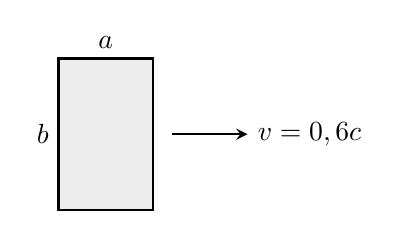
\begin{tikzpicture}[>=stealth, scale=1.2]
  % Ramka
  \draw[thick, fill=gray!15] (0,0) rectangle (1.0, 1.6);
  % Belgilashlar
  \node[above] at (0.5, 1.6) {$a$};
  \node[left] at (0, 0.8) {$b$};
  % Tezlik
  \draw[->, thick] (1.2, 0.8) -- (2.0, 0.8) node[right] {$v = 0,6c$};
\end{tikzpicture}
\end{center}

\begin{enumerate}[label=\Alph*)]
\item 30.
\item 18.
\item 32.
\item 40.
\end{enumerate}

\item Tinchlikdagi uzunligi 20~cm bo‘lgan sterjen rasmdagi kabi $v = \sqrt{3}c/2$ tezlik bilan harakatlanganda, uning uzunligi kuzatuvchiga nisbatan qanday bo‘ladi (cm)?

\begin{center}
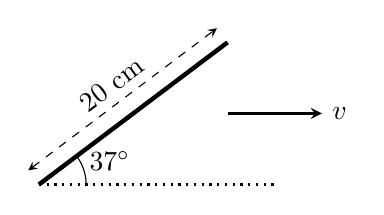
\begin{tikzpicture}[>=stealth, scale=1.5]
  % Gorizontal chiziq
  \draw[dotted, thick] (0,0) -- (2.0,0);
  % Sterjen
  \draw[ultra thick] (0,0) -- ({2.0*cos(37)}, {2.0*sin(37)});
  % Burchak
  \draw (0.4, 0) arc (0:37:0.4);
  \node at (0.6, 0.2) {$37^\circ$};
  % Masofa chizig'i
  \draw[dashed, <->] ({-0.15*sin(37)}, {0.15*cos(37)}) -- ({2.0*cos(37) - 0.15*sin(37)}, {2.0*sin(37) + 0.15*cos(37)});
  \node[above, rotate=37] at ({1.0*cos(37) - 0.15*sin(37)}, {1.0*sin(37) + 0.15*cos(37)}) {20~cm};
  % Tezlik vektori
  \draw[->, thick] ({2.0*cos(37)}, {2.0*sin(37)*0.5}) -- ({2.0*cos(37) + 0.8}, {2.0*sin(37)*0.5}) node[right] {$v$};
\end{tikzpicture}
\end{center}

\begin{enumerate}[label=\Alph*)]
\item $\sqrt{300}$.
\item $\sqrt{208}$.
\item $\sqrt{176}$.
\item 15.
\end{enumerate}

\item Kuzatuvchi bilan bog‘langan sanoq sistemada kometaning harakat yo‘nalishidagi uzunligi, kometaning o‘zi bilan bog‘langan sanoq sistemadagi uzunligi $l_0$ dan $\sqrt{2}$ marta kichik bo‘lsa, kometaning kuzatuvchiga nisbatan tezligi qanday? Yorug‘lik tezligi $c$ ga teng.
\begin{enumerate}[label=\Alph*)]
\item $c/4$.
\item $c/2$.
\item $\sqrt{2}c/2$.
\item $\sqrt{3}c/2$.
\end{enumerate}

\item Tezliklarni qo‘shishning relyativistik qonuni quyidagi ifodalarning qaysi birida to‘g‘ri ko‘rsatilgan?
\begin{enumerate}[label=\Alph*)]
\item $\frac{v_1 v_2}{1+\frac{v_1 v_2}{c^2}}$.
\item $\frac{v_1 / v_2}{1-\frac{v_1 v_2}{c^2}}$.
\item $\frac{v_1 + v_2}{1+\frac{v_1 v_2}{c^2}}$.
\item $\frac{v_1 v_2}{1-\frac{v_1 v_2}{c^2}}$.
\end{enumerate}

\item Yerdan ikkita kosmik kema Yerga nisbatan har biri $0,5c$ tezlik bilan qarama-qarshi tomonga uchirildi. Birinchi kemaning ikkinchisiga nisbatan tezligi qanday?
\begin{enumerate}[label=\Alph*)]
\item $c$.
\item $0$.
\item $0,8c$.
\item $0,5c$.
\end{enumerate}

\item Ikki elektron bir nuqtadan chiqib, shu nuqtaga nisbatan $0,8c$ tezlikda qarama-qarshi tomonga uchib ketdi. Elektronlarning bir-biriga nisbatan tezligini toping.
\begin{enumerate}[label=\Alph*)]
\item $0,8c$.
\item $0,98c$.
\item $0,9c$.
\item $0,95c$.
\end{enumerate}

\item $v$ tezlik bilan harakatlanayotgan kosmik kemadan harakat yo‘nalishida yorug‘lik impulsi yuborildi. Agar bu yorug‘lik impulsining tinch turgan sanoq sistemaga nisbatan tezligi $c$ bo‘lsa, uning kemaga nisbatan tezligi qanday?
\begin{enumerate}[label=\Alph*)]
\item $v$.
\item $c$.
\item $c-v$.
\item $c+v$.
\end{enumerate}

\item Tinchlikdagi massasi $0,3$~g bo‘lgan jismning $0,8c$ tezlik bilan harakatdagi massasini toping (g).
\begin{enumerate}[label=\Alph*)]
\item $0,6$.
\item $0,5$.
\item $0,8$.
\item $1,8$.
\end{enumerate}

\item Tinchlikdagi massasi $4$~kg bo‘lgan jismning harakat vaqtidagi massasi $5$~kg bo‘lsa, uning tezligi qanday? $c$ -- yorug‘likning vakuumdagi tezligi.
\begin{enumerate}[label=\Alph*)]
\item $c$.
\item $0,6c$.
\item $0,4c$.
\item $0,3c$.
\end{enumerate}

\item Tinchlikdagi massasi $m$ bo‘lgan zarraning $0,6c$ tezlik bilan harakatlanayotganidagi massasini toping.
\begin{enumerate}[label=\Alph*)]
\item $1,83m$.
\item $1,67m$.
\item $1,25m$.
\item $1,56m$.
\end{enumerate}

\item Tezligi $0,87c$ bo‘lgan elektronning massasi uning tinchlikdagi massasidan necha marta katta?
\begin{enumerate}[label=\Alph*)]
\item $2$.
\item $2,5$.
\item $4$.
\item $5$.
\end{enumerate}

\item Ushbu rasmdagi parallelopiped shaklidagi jism qanday tezlik bilan harakatlansa, uning hajmi $10$~m$^3$ bo‘lib qoladi?

\begin{center}
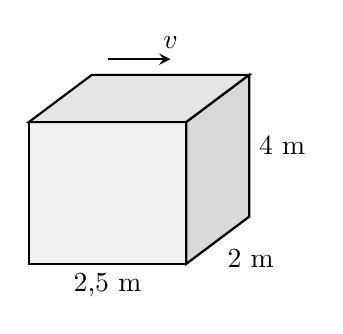
\begin{tikzpicture}[>=stealth]
  % 3D Jism
  \draw[thick, fill=gray!10] (0,0) rectangle (2.0, 1.8);
  \draw[thick, fill=gray!20] (0, 1.8) -- (0.8, 2.4) -- (2.8, 2.4) -- (2.0, 1.8) -- cycle;
  \draw[thick, fill=gray!30] (2.0, 0) -- (2.8, 0.6) -- (2.8, 2.4) -- (2.0, 1.8) -- cycle;
  % O'lchamlar
  \node[below] at (1.0, 0) {2,5~m};
  \node[right] at (2.8, 1.5) {4~m};
  \node[below right] at (2.4, 0.3) {2~m};
  % Tezlik ko'rsatkichi
  \draw[->, thick] (1.0, 2.6) -- (1.8, 2.6) node[above] {$v$};
\end{tikzpicture}
\end{center}

\begin{enumerate}[label=\Alph*)]
\item $c/4$.
\item $c/2$.
\item $\sqrt{3}c/4$.
\item $\sqrt{3}c/2$.
\end{enumerate}

\item Yorug‘lik tezligiga yaqin tezlikda harakatlanayotgan jismning chiziqli o‘lchami harakat yo‘nalishida $1,2$ marta kamaysa, uning hajmi qanday o‘zgaradi?
\begin{enumerate}[label=\Alph*)]
\item o‘zgarmaydi.
\item $1,2$ marta ortadi.
\item $1,728$ marta kamayadi.
\item $1,2$ marta kamayadi.
\end{enumerate}

\item Nyuton mexanikasi qonunlari hamma vaqt o‘rinlimi?
\begin{enumerate}[label=\Alph*)]
\item Yo‘q! Faqatgina jismlarning tezligi yorug‘lik tezligidan juda kichik bo‘lganidagina o‘rinli.
\item Hamma vaqt emas, faqat inersial sanoq sistemalarda o‘rinli.
\item Hamisha emas, faqat muayyan sanoq sistemadagina o‘rinli.
\item Hamma vaqt emas, faqat tinch holatdagi sanoq sistemalarda o‘rinli.
\end{enumerate}

\end{enumerate}\



\begin{table}[!ht]
\centering
\begin{tabular}{|c|c|c|c|c|c|c|c|c|c|c|}
\hline
1b & 2b & 3c & 4d & 5d & 6d & 7b & 8c & 9c & 10c & 11b \\ \hline
12b & 13b & 14b & 15c & 16a & 17d & 18d & 19a & & & \\ \hline
\end{tabular}
\end{table}